\documentclass[11pt,a4paper]{article}
\newcommand{\intestazione}{Dimero di spin --- 1. Il sistema}
% =====================================================================
%  Preambolo comune ai documenti sul dimero (serie "che cosa abbiamo fatto")
%  Incluso con % =====================================================================
%  Preambolo comune ai documenti sul dimero (serie "che cosa abbiamo fatto")
%  Incluso con % =====================================================================
%  Preambolo comune ai documenti sul dimero (serie "che cosa abbiamo fatto")
%  Incluso con \input{preambolo_dimero} subito dopo \documentclass.
% =====================================================================
\usepackage[T1]{fontenc}
\usepackage[utf8]{inputenc}
\usepackage[main=italian,provide=*]{babel}
\usepackage{amsmath,amssymb,mathtools}
\usepackage{graphicx}
\usepackage{booktabs}
\usepackage{colortbl}
\usepackage{xcolor}
\usepackage{geometry}
\usepackage{placeins}
\usepackage{caption}
\usepackage{enumitem}
\usepackage{fancyhdr}
\usepackage{needspace}
\usepackage{tikz}
\usetikzlibrary{arrows.meta,positioning,shapes.geometric,calc,fit,backgrounds}
\usepackage{hyperref}
\hypersetup{colorlinks=true,linkcolor=blu,citecolor=blu,urlcolor=blu}

\geometry{margin=2.5cm}

% --- colori coerenti con quelli delle figure (palette Okabe-Ito)
\definecolor{blu}{HTML}{0072B2}
\definecolor{arancio}{HTML}{E69F00}
\definecolor{verdes}{HTML}{009E73}
\definecolor{rossos}{HTML}{D55E00}
\definecolor{violas}{HTML}{CC79A7}
\definecolor{grigetto}{HTML}{E8E8E8}

\captionsetup{font=small,labelfont=bf,width=0.92\textwidth}

\pagestyle{fancy}
\fancyhf{}
\fancyhead[L]{\small\itshape\intestazione}
\fancyhead[R]{\small\thepage}
\renewcommand{\headrulewidth}{0.3pt}

% --- notazione
\newcommand{\ket}[1]{\lvert #1\rangle}
\newcommand{\bra}[1]{\langle #1 \rvert}
\newcommand{\media}[1]{\langle #1 \rangle}
\newcommand{\vs}[1]{\mathbf{s}_{#1}}

% --- riquadro "in una riga": il messaggio da portare a casa
\newcommand{\messaggio}[1]{%
  \begin{center}
  \begin{minipage}{0.93\textwidth}
  \setlength{\fboxsep}{9pt}%
  \colorbox{grigetto}{\begin{minipage}{\dimexpr\textwidth-2\fboxsep}
  \small\textbf{In una riga.}\enspace #1
  \end{minipage}}
  \end{minipage}
  \end{center}
}

% --- riquadro "come lo sappiamo": la verifica numerica dietro un'affermazione
\newcommand{\verifica}[1]{%
  \begin{center}
  \begin{minipage}{0.93\textwidth}
  \small\textcolor{verdes}{\rule{2.2em}{1.1pt}}\enspace
  \textcolor{verdes}{\textbf{Come lo sappiamo.}}\enspace #1
  \end{minipage}
  \end{center}
  \medskip
}
 subito dopo \documentclass.
% =====================================================================
\usepackage[T1]{fontenc}
\usepackage[utf8]{inputenc}
\usepackage[main=italian,provide=*]{babel}
\usepackage{amsmath,amssymb,mathtools}
\usepackage{graphicx}
\usepackage{booktabs}
\usepackage{colortbl}
\usepackage{xcolor}
\usepackage{geometry}
\usepackage{placeins}
\usepackage{caption}
\usepackage{enumitem}
\usepackage{fancyhdr}
\usepackage{needspace}
\usepackage{tikz}
\usetikzlibrary{arrows.meta,positioning,shapes.geometric,calc,fit,backgrounds}
\usepackage{hyperref}
\hypersetup{colorlinks=true,linkcolor=blu,citecolor=blu,urlcolor=blu}

\geometry{margin=2.5cm}

% --- colori coerenti con quelli delle figure (palette Okabe-Ito)
\definecolor{blu}{HTML}{0072B2}
\definecolor{arancio}{HTML}{E69F00}
\definecolor{verdes}{HTML}{009E73}
\definecolor{rossos}{HTML}{D55E00}
\definecolor{violas}{HTML}{CC79A7}
\definecolor{grigetto}{HTML}{E8E8E8}

\captionsetup{font=small,labelfont=bf,width=0.92\textwidth}

\pagestyle{fancy}
\fancyhf{}
\fancyhead[L]{\small\itshape\intestazione}
\fancyhead[R]{\small\thepage}
\renewcommand{\headrulewidth}{0.3pt}

% --- notazione
\newcommand{\ket}[1]{\lvert #1\rangle}
\newcommand{\bra}[1]{\langle #1 \rvert}
\newcommand{\media}[1]{\langle #1 \rangle}
\newcommand{\vs}[1]{\mathbf{s}_{#1}}

% --- riquadro "in una riga": il messaggio da portare a casa
\newcommand{\messaggio}[1]{%
  \begin{center}
  \begin{minipage}{0.93\textwidth}
  \setlength{\fboxsep}{9pt}%
  \colorbox{grigetto}{\begin{minipage}{\dimexpr\textwidth-2\fboxsep}
  \small\textbf{In una riga.}\enspace #1
  \end{minipage}}
  \end{minipage}
  \end{center}
}

% --- riquadro "come lo sappiamo": la verifica numerica dietro un'affermazione
\newcommand{\verifica}[1]{%
  \begin{center}
  \begin{minipage}{0.93\textwidth}
  \small\textcolor{verdes}{\rule{2.2em}{1.1pt}}\enspace
  \textcolor{verdes}{\textbf{Come lo sappiamo.}}\enspace #1
  \end{minipage}
  \end{center}
  \medskip
}
 subito dopo \documentclass.
% =====================================================================
\usepackage[T1]{fontenc}
\usepackage[utf8]{inputenc}
\usepackage[main=italian,provide=*]{babel}
\usepackage{amsmath,amssymb,mathtools}
\usepackage{graphicx}
\usepackage{booktabs}
\usepackage{colortbl}
\usepackage{xcolor}
\usepackage{geometry}
\usepackage{placeins}
\usepackage{caption}
\usepackage{enumitem}
\usepackage{fancyhdr}
\usepackage{needspace}
\usepackage{tikz}
\usetikzlibrary{arrows.meta,positioning,shapes.geometric,calc,fit,backgrounds}
\usepackage{hyperref}
\hypersetup{colorlinks=true,linkcolor=blu,citecolor=blu,urlcolor=blu}

\geometry{margin=2.5cm}

% --- colori coerenti con quelli delle figure (palette Okabe-Ito)
\definecolor{blu}{HTML}{0072B2}
\definecolor{arancio}{HTML}{E69F00}
\definecolor{verdes}{HTML}{009E73}
\definecolor{rossos}{HTML}{D55E00}
\definecolor{violas}{HTML}{CC79A7}
\definecolor{grigetto}{HTML}{E8E8E8}

\captionsetup{font=small,labelfont=bf,width=0.92\textwidth}

\pagestyle{fancy}
\fancyhf{}
\fancyhead[L]{\small\itshape\intestazione}
\fancyhead[R]{\small\thepage}
\renewcommand{\headrulewidth}{0.3pt}

% --- notazione
\newcommand{\ket}[1]{\lvert #1\rangle}
\newcommand{\bra}[1]{\langle #1 \rvert}
\newcommand{\media}[1]{\langle #1 \rangle}
\newcommand{\vs}[1]{\mathbf{s}_{#1}}

% --- riquadro "in una riga": il messaggio da portare a casa
\newcommand{\messaggio}[1]{%
  \begin{center}
  \begin{minipage}{0.93\textwidth}
  \setlength{\fboxsep}{9pt}%
  \colorbox{grigetto}{\begin{minipage}{\dimexpr\textwidth-2\fboxsep}
  \small\textbf{In una riga.}\enspace #1
  \end{minipage}}
  \end{minipage}
  \end{center}
}

% --- riquadro "come lo sappiamo": la verifica numerica dietro un'affermazione
\newcommand{\verifica}[1]{%
  \begin{center}
  \begin{minipage}{0.93\textwidth}
  \small\textcolor{verdes}{\rule{2.2em}{1.1pt}}\enspace
  \textcolor{verdes}{\textbf{Come lo sappiamo.}}\enspace #1
  \end{minipage}
  \end{center}
  \medskip
}


\title{\bfseries Il sistema: due spin, quattro livelli, un incrocio\\[2pt]
\large Documento 1 --- che cosa c'è da simulare, e perché non è banale}
\author{Samuele Schiavi \\ \small Tesi triennale in Fisica, Università di Parma
--- Relatore: Prof.\ Alessandro Chiesa}
\date{}

\begin{document}
\maketitle
\thispagestyle{fancy}

\section{Il punto di partenza}

Due spin $1/2$ accoppiati, immersi in un campo magnetico lungo $z$. Il modello,
nella convenzione usata in tutto il progetto, è
\begin{equation}
H = J\,(X_1X_2+Y_1Y_2+Z_1Z_2) + b\,(Z_1+Z_2) + D\,(X_1Z_2-Z_1X_2),
\label{eq:H}
\end{equation}
dove $X_i,Y_i,Z_i$ sono le matrici di Pauli sul sito $i$. I primi due termini
descrivono uno scambio di Heisenberg isotropo e l'accoppiamento Zeeman col
campo; il terzo, antisimmetrico, è un termine di Dzyaloshinskii--Moriya (DM). Il
parametro di controllo naturale è il rapporto $b/J$: nelle figure che seguono
$J=1$ e il campo varia.

Il fatto che rende questo sistema il punto di partenza giusto per una tesi sul
calcolo quantistico è la corrispondenza uno-a-uno fra spin e qubit. Un elettrone
in una molecola richiederebbe una trasformazione fermionica e decine di qubit;
uno spin $1/2$ \emph{è} già un qubit. Due spin, due qubit.

\section{Lo spettro, e dove diventa interessante}

Con $D=0$ il problema si risolve in forma chiusa: gli autovalori dipendono solo
dallo spin totale $S$ e dalla sua proiezione $M$,
\begin{equation}
E(S,M) = 2J\,S(S{+}1) - 3J + 2bM .
\end{equation}
Quattro stati: un singoletto ($S=0$, energia $-3J$, indipendente dal campo) e un
tripletto ($S=1$), le cui tre componenti si separano linearmente in $b$.

\begin{figure}[htbp]
\centering
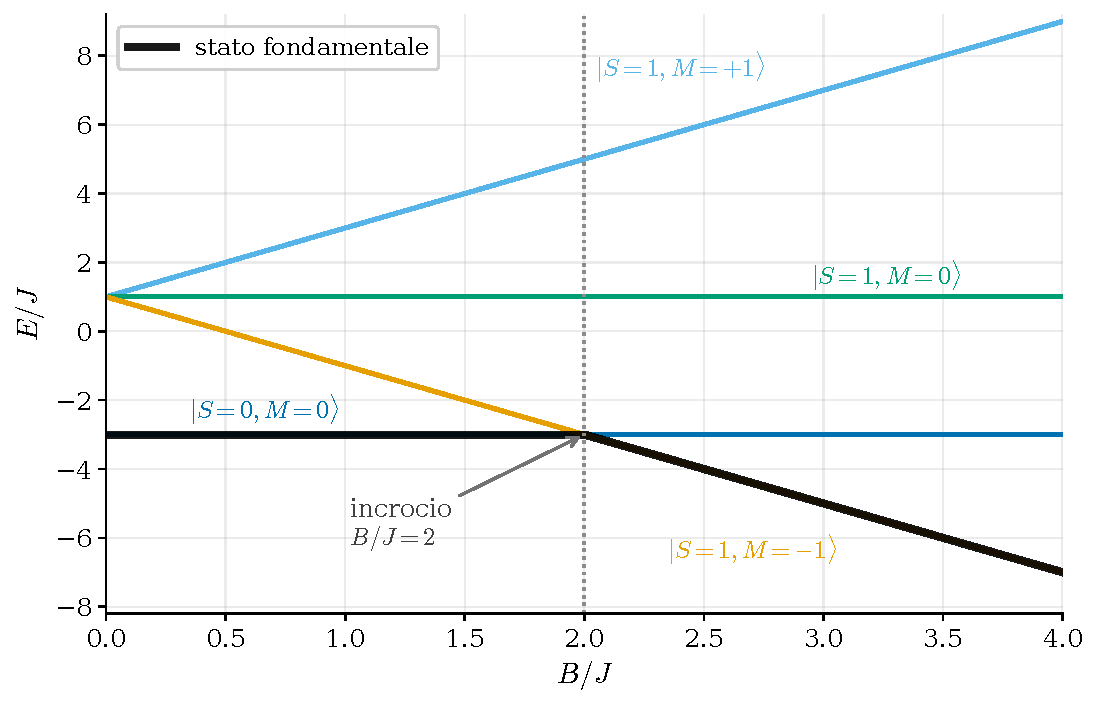
\includegraphics[width=0.86\textwidth]{figure/fig01_spettro}
\caption{I quattro livelli in funzione del campo, per $D=0$. Il singoletto
(blu) non risente del campo; le tre componenti del tripletto si aprono a
ventaglio. La curva nera spessa segue lo stato di energia più bassa: fino a
$B/J=2$ è il singoletto, oltre diventa la componente $M=-1$ del tripletto. Nel
punto di scambio le due rette si attraversano senza deviare: è un incrocio vero,
non un avvicinamento.}
\label{fig:spettro}
\end{figure}

\FloatBarrier

La struttura è semplice ma contiene già il problema centrale. A $B/J=2$ lo stato
fondamentale cambia identità di colpo: il sistema passa da uno stato
completamente entangled (il singoletto) a uno stato di prodotto
($\ket{\!\downarrow\downarrow}$). Nel punto di incrocio i due sono degeneri, e
``lo stato fondamentale'' cessa di essere un oggetto ben definito --- qualunque
loro combinazione ha la stessa energia.

\messaggio{L'incrocio a $B/J=2$ non è un dettaglio dello spettro: è il punto in
cui la domanda ``qual è lo stato fondamentale?'' non ha una risposta unica, e
quindi il punto in cui ogni metodo variazionale rischia di rompersi.}

\section{Perché l'incrocio non si apre da solo}

I due stati che si incrociano hanno magnetizzazione diversa: $M=0$ il
singoletto, $M=-1$ il tripletto basso. Finché l'Hamiltoniana conserva $M$ --- e
i primi due termini della \eqref{eq:H} lo fanno --- l'elemento di matrice che li
collegherebbe è nullo per ragioni di simmetria, non per un accidente numerico:
\begin{equation}
\bra{S{=}0,M{=}0}\,H_{\text{isotropo}}+H_{\text{campo}}\,\ket{S{=}1,M{=}{-}1} = 0 .
\end{equation}
Senza accoppiamento, le due curve si attraversano. Per aprire l'incrocio serve
un termine che connetta settori di $M$ diversi. È esattamente il ruolo del
termine DM.

\needspace{9\baselineskip}
\section{Che cosa fa concretamente il termine DM}

Il DM non conserva la magnetizzazione. Il modo diretto di verificarlo è
misurare quanto ``non commuta'':
\begin{equation}
\lVert [H_D, S_z] \rVert = 0.566, \qquad
\lVert [H_D, S^2] \rVert = 1.131 \qquad (D=0.2,\ \text{norma di Frobenius}).
\end{equation}
Entrambi diversi da zero: il termine può mescolare stati con $M$ diverso, e
quindi può aprire l'incrocio. L'effetto si vede su due osservabili distinte.

\begin{figure}[htbp]
\centering
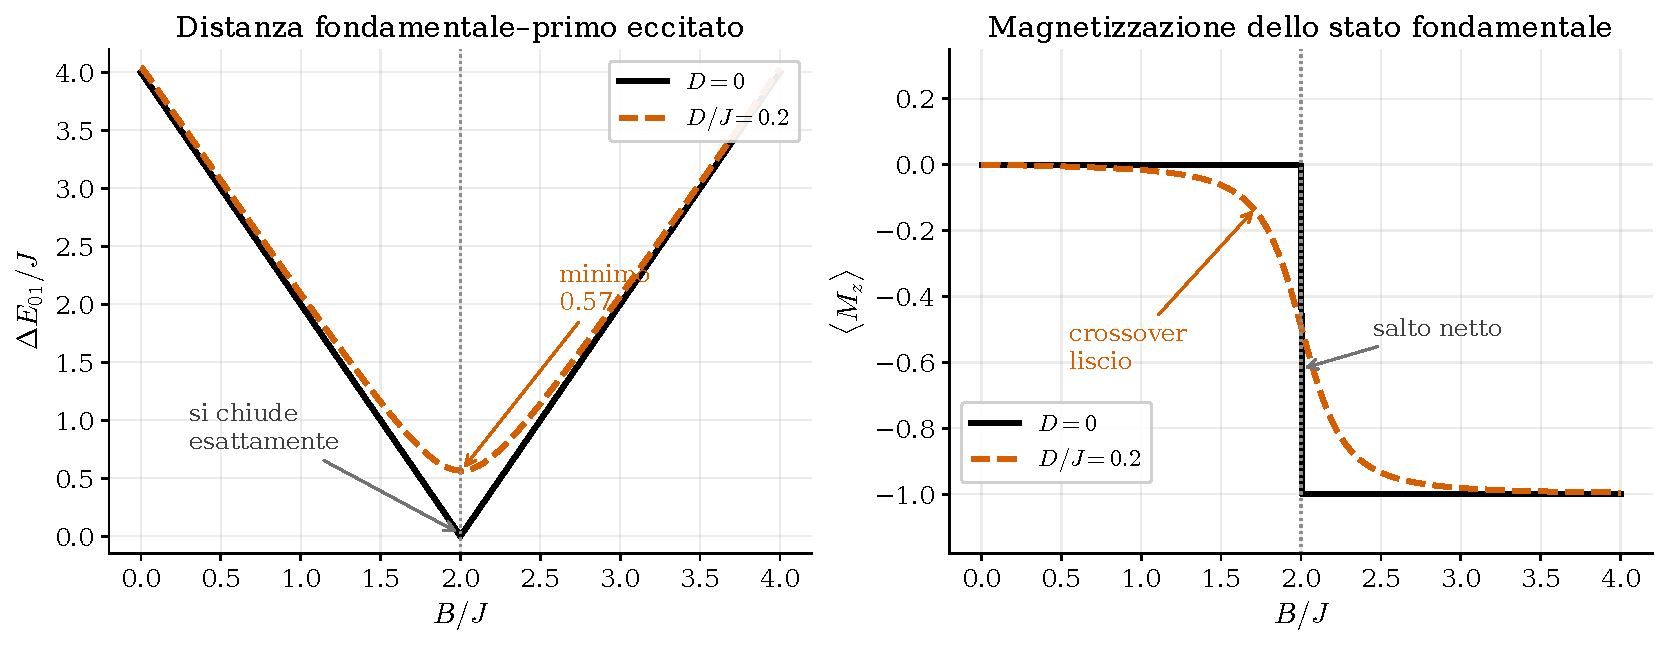
\includegraphics[width=\textwidth]{figure/fig02_gap_magnetizzazione}
\caption{\textbf{A sinistra:} la distanza fra stato fondamentale e primo stato
eccitato. Con $D=0$ (nero) si annulla esattamente a $B/J=2$; con $D/J=0.2$
(arancio tratteggiato) resta finita, con un minimo di $0.565$. \textbf{A
destra:} la magnetizzazione dello stato fondamentale. Il salto netto da $0$ a
$-1$ diventa un crossover continuo. È la firma osservabile dello stesso
fenomeno: dove i livelli non si toccano più, lo stato fondamentale cambia con
continuità invece che di scatto.}
\label{fig:gap}
\end{figure}

\FloatBarrier

\verifica{I valori del gap sono ricalcolati diagonalizzando la matrice
$4\times4$ su una griglia di $601$ punti in $b$. A $B/J=2$: gap $=0.000$ per
$D=0$, gap $=0.565$ per $D/J=0.2$. Il minimo del gap con DM cade a $B/J=2.007$,
non esattamente a $2$ --- il DM sposta leggermente il punto oltre ad aprirlo.
Lo spettro numerico coincide con la formula analitica a $D=0$ con scarto
massimo $8.9\times10^{-16}$.}

\section{Perché questo conta per il resto del lavoro}

C'è una tentazione, guardando la figura~\ref{fig:gap}, di leggere il termine DM
come una complicazione aggiunta per realismo. Non è così, e vale la pena essere
precisi sul suo ruolo, perché è il filo che regge i tre documenti successivi.

\begin{enumerate}[leftmargin=1.5em,itemsep=4pt]
\item \textbf{Rende ben posto il problema variazionale.} Un algoritmo che cerca
lo stato di energia minima ha bisogno che quello stato sia unico. Con l'incrocio
aperto, lo è su tutto il range di campo, e la fidelity rispetto al riferimento
esatto diventa una quantità con un significato non ambiguo.

\item \textbf{Rompe la simmetria su cui gli ansatz efficienti sono costruiti.}
Questo è il punto meno ovvio. Costruire un circuito parametrico che rispetti la
conservazione di $M$ è enormemente conveniente --- servono pochissimi parametri.
Ma se l'Hamiltoniana non conserva $M$, quel circuito non può raggiungere il suo
stato fondamentale, per quanti parametri gli si aggiungano. È il contenuto del
documento 2.

\item \textbf{Impedisce la fattorizzazione esatta dell'evoluzione temporale.}
Con $D=0$ i pezzi dell'Hamiltoniana commutano e $e^{-iHt}$ si scrive
esattamente come prodotto di blocchi semplici. Con $D\neq0$ non commutano più, e
serve un'approssimazione controllata --- la decomposizione di Suzuki--Trotter.
È il contenuto del documento 3.
\end{enumerate}

\messaggio{Una precisazione terminologica che conviene tenere pronta: qui si
parla di rottura \emph{esplicita} di una simmetria --- un termine aggiunto
all'Hamiltoniana --- non di rottura spontanea. Lo stato fondamentale non è meno
simmetrico dell'Hamiltoniana: è l'Hamiltoniana stessa a non avere più quella
simmetria.}

\end{document}
